\capitulo{4}{Técnicas y herramientas}

A lo largo del desarrollo del proyecto, se han empleado diversas tecnologías, herramientas y elementos esenciales que requieren familiaridad antes de avanzar en la ejecución del proyecto. La elección de estas opciones en lugar de otras se basa en una evaluación detallada, la cual queda documentada en esta sección con el propósito de brindar una justificación fundamentada.

\section{Entorno Software}
\subsection{Entorno de desarrollo Micropython}\label{4:MicroPython}
%Thonny~\cite{misc:Thonny} 
\begin{itemize}
	\item \textbf{Herramientas valoradas:} \href{https://thonny.org/}{Thonny IDE}, \href{https://codewith.mu/}{Mu Editor}, \href{https://dfrobot.gitbooks.io/upycraft/content/}{Upycraft}, \href{https://www.jetbrains.com/pycharm/}{PyCharm}.
    \item \textbf{Herramienta elegida:} \href{https://thonny.org/}{Thonny IDE}.
\end{itemize}

Thonny IDE se presenta como la opción más idónea, proporcionando una combinación de simplicidad, integración nativa con MicroPython, herramientas de depuración eficaces y un sólido soporte comunitario, todo lo cual contribuye a un entorno de desarrollo eficiente y centrado en el usuario para la programación en la Raspberry Pi Pico W con MicroPython.

\begin{figure}[h]
    \centering
    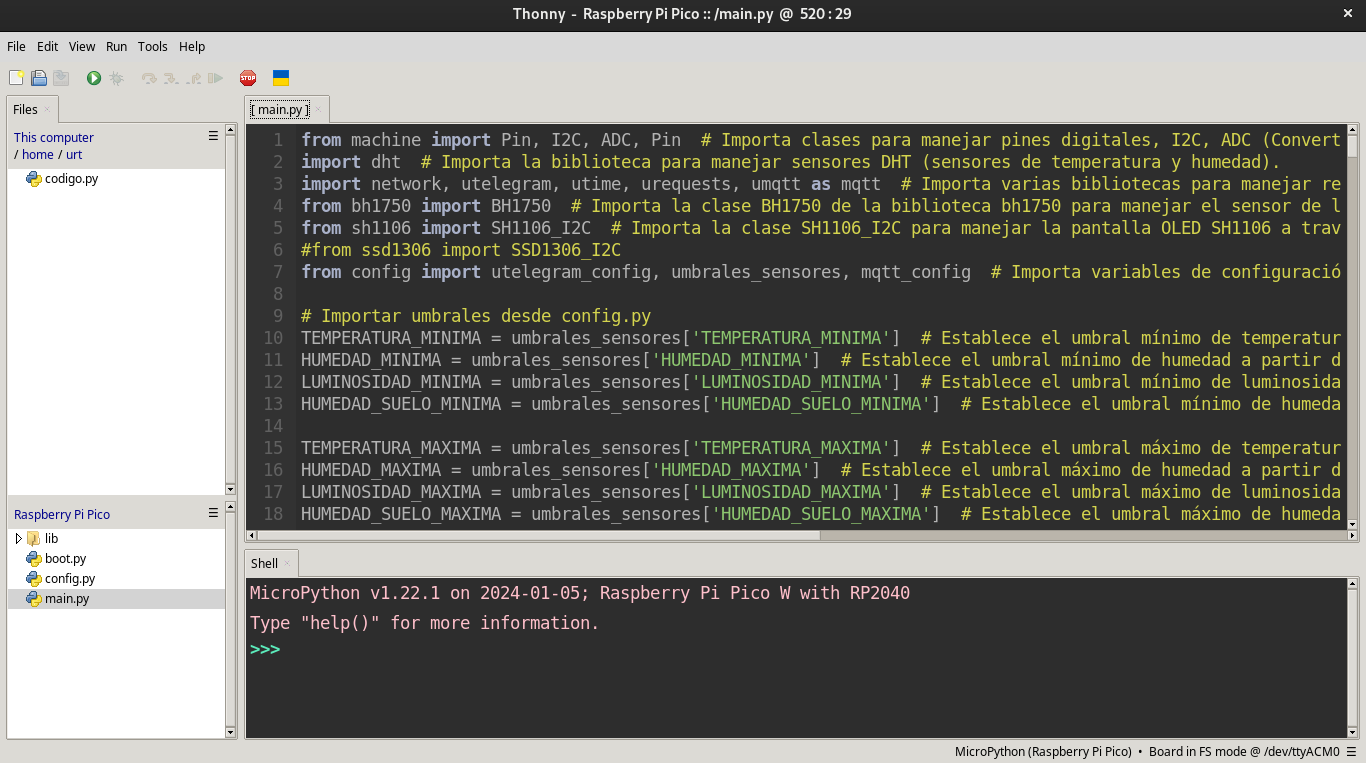
\includegraphics[width=1\textwidth]{img/herramientas/thonny.png}
    \caption{IDE Thonny.} \label{Img:Thonny}
\end{figure}
 \pagebreak

\subsection{Entorno de desarrollo Python}\label{4:Python}
\begin{itemize}
    \item \textbf{Herramientas valoradas:} \href{https://colab.google/}{Google colab} y \href{https://jupyter.org/}{Jupyter Notebook}.
    \item \textbf{Herramienta elegida:} \href{https://jupyter.org/}{Jupyter Notebook}.
\end{itemize}

Jupyter Notebook~\cite{misc:Jupyter_Notebook} es una herramienta de código abierto poderosa que facilita la creación y compartición de documentos interactivos. Estos documentos pueden contener código ejecutable, visualizaciones, texto narrativo y otros elementos. Opto por utilizar Jupyter Notebook en mi Trabajo de Fin de Grado debido a su versatilidad y capacidad para aprovechar los entornos virtuales que he configurado en mi computadora. Este entorno se ha vuelto fundamental para llevar a cabo análisis de datos, especialmente haciendo uso intensivo de la biblioteca Pandas~\cite{misc:Pandas} para manipulación y procesamiento de datos.
%\begin{figure}[h]
    %\centering
    %
\includegraphics[width=0.1\textwidth]{img/herramientas/jupyter_logo.png}
    %\caption{Jupyter logo.} \label{Img:Jupyter}
%\end{figure}
\pagebreak
\section{Control de datos}
\subsection{APIS}\label{4:APIS}
\begin{itemize}
    \item \textbf{API de Telegram:}
La API de Telegram~\cite{misc:Telegram_api}, accesible a través de la URL \url{https://api.telegram.org/bot<token>}, juega un papel fundamental en la integración de bots de Telegram~\cite{misc:Telegram_bots} con el sistema. Permite la interacción bidireccional entre el sistema y los usuarios a través de la plataforma de mensajería Telegram. Al utilizar esta API, se establece una conexión segura para enviar y recibir mensajes, comandos y datos entre el sistema y los usuarios mediante la implementación de funciones específicas proporcionadas por Telegram. Esto posibilita la notificación remota, la recopilación de datos y la activación de acciones automatizadas, contribuyendo así a la funcionalidad integral del sistema de control de datos.
Esta API fue usada en el código MicroPython.
    \item \textbf{API WorldTime}\label{4:API_Hora}
		La API de WorldTime~\cite{misc:WorlTimeAPI}, accesible mediante la URL \url{http://worldtimeapi.org/api/ip}, ofrece información precisa sobre la hora mundial basada en la ubicación asociada a la dirección IP del usuario. Al realizar una solicitud a esta API, se obtiene información detallada sobre la hora actual, la fecha, el huso horario y otros datos relacionados con la hora en la ubicación correspondiente a la dirección IP consultada. Esta API es valiosa para aplicaciones que requieren sincronización horaria precisa y la visualización de la hora actual en diferentes regiones del mundo. Su facilidad de acceso y respuesta estructurada la convierten en una herramienta útil para integrar la información horaria global en aplicaciones y sistemas.
Esta API fue usada en el código MicroPython.
\end{itemize}
\pagebreak

\section{Entorno Hardware}
\subsection{Fritzing}
Fritzing~\cite{misc:Fritzing} es una herramienta de diseño electrónico de código abierto que facilita la creación de esquemas, prototipos y layouts de placas de circuito impreso (PCB). Diseñado para usuarios, desde principiantes hasta expertos, Fritzing ofrece una interfaz intuitiva y gráfica que permite la conexión visual de componentes electrónicos, como sensores, actuadores y placas de desarrollo. Su funcionalidad principal abarca desde la creación de esquemas eléctricos hasta la generación de archivos Gerber para la fabricación de PCB. Fritzing se destaca por su accesibilidad y capacidad para convertir conceptos de diseño en proyectos electrónicos tangibles, lo que lo convierte en una herramienta valiosa para ingenieros, diseñadores y entusiastas que desean visualizar y materializar sus ideas electrónicas.
\begin{figure}[h]
    \centering
    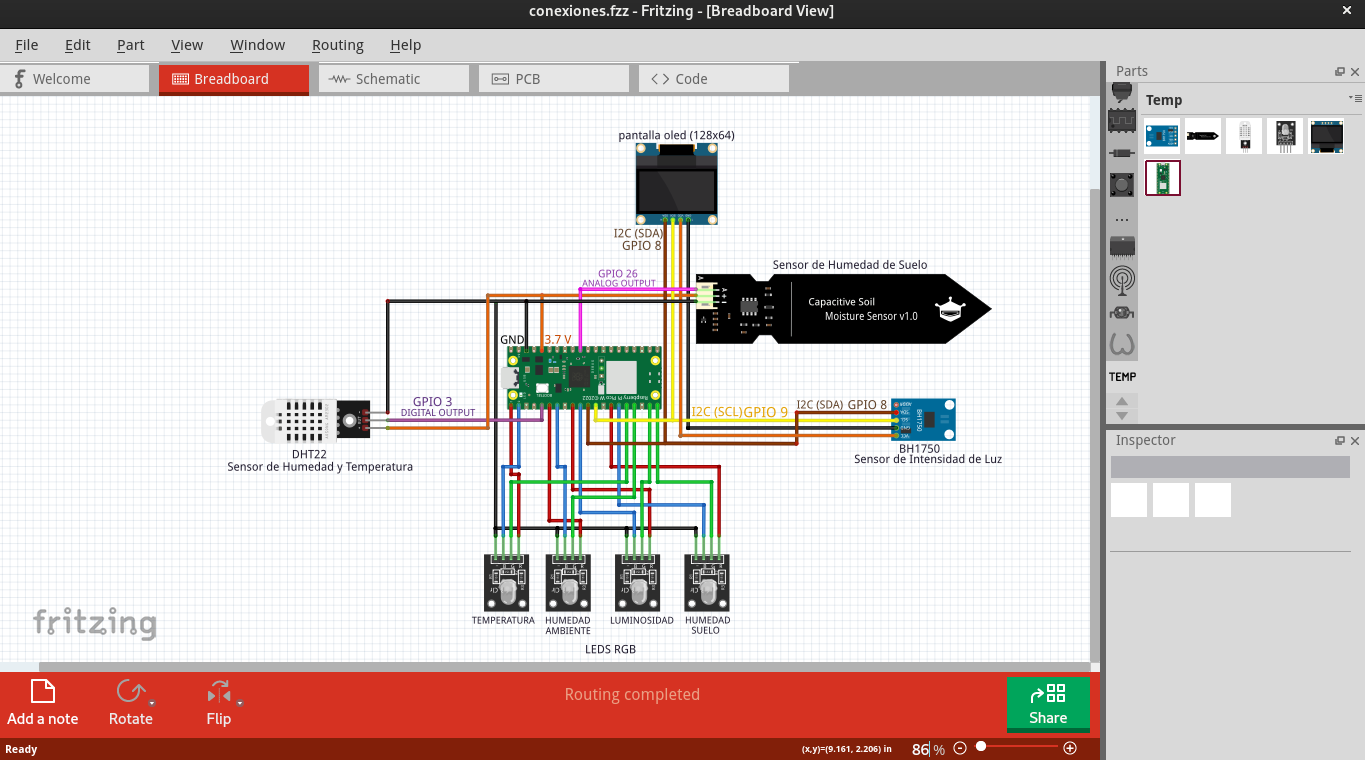
\includegraphics[width=1\textwidth]{img/herramientas/fritzing.png}
    \caption{Esquema de conexiones diseñado con Fritzing.}
\end{figure}
\pagebreak

\section{Metodologías}
\subsection{Modularidad}
La modularidad es un principio clave en la metodología de desarrollo que implica la división de un sistema en módulos independientes y autónomos, cada uno de los cuales realiza una función específica y bien definida. En el contexto del diseño de un sistema económico IoT para la monitorización de invernaderos de cannabis medicinal, la aplicación de la modularidad implica organizar el software y el hardware en componentes distintos y fácilmente intercambiables.

Características de la Modularidad:

\begin{itemize}
\item \textbf{Independencia Funcional:}
Cada módulo opera de forma independiente, realizando una tarea específica sin depender excesivamente de otros. Esto facilita la comprensión individual y la posibilidad de actualizar o cambiar un módulo sin afectar el funcionamiento general.

\item \textbf{Interconexión Estandarizada:}
Aunque los módulos operan de manera independiente, la interconexión entre ellos sigue estándares predefinidos. Esto facilita la comunicación y la interoperabilidad entre los componentes del sistema.

\item \textbf{Facilita el Mantenimiento:}
La modularidad simplifica el mantenimiento del sistema, ya que las actualizaciones o correcciones pueden realizarse en módulos específicos sin afectar otras partes del sistema. Esto mejora la capacidad de respuesta y reduce el riesgo de errores inadvertidos.

\item \textbf{Escalabilidad:}
La estructura modular permite una fácil escalabilidad del sistema. Se pueden agregar nuevos módulos o funciones sin afectar negativamente la estructura existente, lo que facilita la adaptación del sistema a cambios futuros.

\item \textbf{Reutilización de Componentes:}
Los módulos pueden diseñarse para ser reutilizables en diferentes partes del proyecto o incluso en proyectos futuros. Esto reduce la redundancia y fomenta la eficiencia en el desarrollo.

\item \textbf{Facilita la Colaboración:}
La división en módulos facilita la colaboración entre diferentes equipos o desarrolladores, ya que cada grupo puede trabajar de manera independiente en su propio módulo, siempre y cuando se respeten las interfaces definidas.
\end{itemize}

\begin{figure}[h]
    \centering
    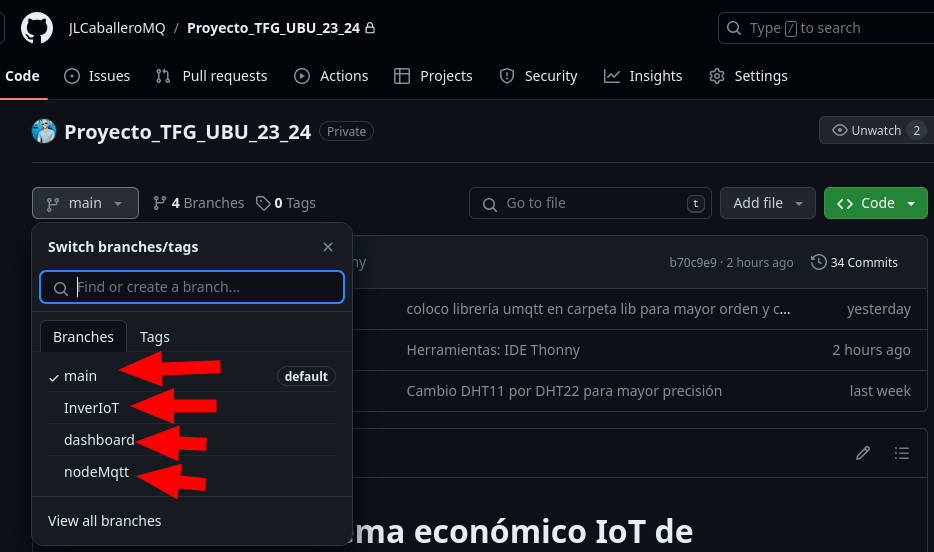
\includegraphics[width=1\textwidth]{img/desarrollo/modularidad.png}
	\caption{Estructura de ramas en GitHub aplicando modularidad. }
\end{figure}
Cada rama representa un módulo o característica específica del proyecto, permitiendo un desarrollo paralelo y aislado. Las ramas se fusionan con la rama principal una vez que las funcionalidades están completas y probadas. Esta estrategia facilita la gestión modular del proyecto y la colaboración entre desarrolladores.

\section{Entorno de desarrollo del Proyecto}
\subsection{Control de versiones o CVS, Concurrent Versioning System}\label{4:controlVersiones}
\begin{itemize}
    \item \textbf{Herramientas valoradas:} \href{https://git-scm.com/}{Git}, \href{https://subversion.apache.org/}{SVN}.
    \item \textbf{Herramienta elegida:} \href{https://git-scm.com/}{Git}.
\end{itemize}
Git~\cite{misc:Git} es un sistema de control de versiones distribuido, ampliamente utilizado en el desarrollo de software y es conocido por su velocidad, flexibilidad y eficiencia en la gestión de versiones de código fuente.

Comparación con SVN:

Subversion (SVN)~\cite{misc:SVN} es otro sistema de control de versiones, pero sigue un modelo centralizado, a diferencia del modelo distribuido de Git. Aquí hay algunas diferencias clave y ventajas de Git sobre SVN:
\begin{itemize}
	\item \textbf{Descentralización:}
Git es completamente descentralizado, lo que significa que cada usuario tiene una copia completa del repositorio con todo su historial. En SVN, los usuarios dependen del servidor central para muchas operaciones.

\item \textbf{Ramificación y Fusiones Rápidas:}
Git permite ramificaciones ligeras y fusiones rápidas, lo que facilita el desarrollo paralelo y la gestión de características en diferentes ramas. SVN maneja ramificaciones y fusiones, pero históricamente ha sido menos eficiente en comparación con Git.

\item \textbf{Eficiencia en Red:}
Git es más eficiente en términos de ancho de banda y operaciones de red, ya que las operaciones se realizan localmente en la mayoría de los casos. SVN, al depender más del servidor central, puede ser más lento en operaciones que implican la red.

\item \textbf{Historial Completo y Offline:}
Git almacena el historial completo localmente, lo que permite el trabajo fuera de línea. SVN requiere acceso al servidor para recuperar el historial completo.

\item \textbf{Flexibilidad y Escalabilidad:}
Git es conocido por su flexibilidad y escalabilidad, especialmente en proyectos grandes y complejos. SVN puede encontrar limitaciones en proyectos extensos y complejos.
\end{itemize}


\subsection{Hosting del Repositorio}
\begin{itemize}
    \item \textbf{Herramientas valoradas:} \href{https://github.com/}{Github} y \href{https://bitbucket.org/product/}{Bitbucket}.
    \item \textbf{Herramienta elegida:} \href{https://github.com/}{Github}.
\end{itemize}
GitHub~\cite{misc:Github} es una plataforma de desarrollo colaborativo basada en Git que facilita el alojamiento y la colaboración en proyectos de software. 

Bitbucket~\cite{misc:Bitbucket} es otra plataforma de desarrollo colaborativo basada en Git, pero hay algunas diferencias clave. Aquí se exploran estas diferencias y se destaca una ventaja de GitHub sobre Bitbucket:

\begin{itemize}
	\item \textbf{Visibilidad del Código Fuente:}
		GitHub ha sido históricamente más popular para proyectos de código abierto, y los repositorios públicos en GitHub suelen tener una mayor visibilidad y participación de la comunidad en comparación con Bitbucket.

\item \textbf{Comunidad y Desarrollo Abierto:}
GitHub se ha convertido en el estándar de facto para proyectos de código abierto, y muchos desarrolladores buscan activamente proyectos en GitHub. Esto hace que sea más fácil para los proyectos atraer colaboradores y contribuyentes.

\item \textbf{Integraciones y Ecosistema:}
GitHub tiene una amplia gama de integraciones y herramientas de terceros que son ampliamente utilizadas en la comunidad de desarrollo. La rica integración con servicios como Travis CI, CircleCI y otros facilita el desarrollo y la automatización.

\item \textbf{Herramientas de Colaboración:}
Mientras que Bitbucket ofrece características similares, GitHub es generalmente preferido por su interfaz de usuario intuitiva, herramientas de revisión de código más robustas y una experiencia general más pulida para la colaboración.

\item \textbf{Repositorios Públicos Gratuitos:}
GitHub permite la creación de repositorios públicos de forma gratuita, lo que fomenta la participación y el desarrollo colaborativo en proyectos de código abierto. Bitbucket, por otro lado, suele ofrecer repositorios privados gratuitos, pero limita la cantidad de colaboradores.
\end{itemize}


\subsection{Editor del proyecto}\label{4:ATOM}
\begin{itemize}
    \item \textbf{Herramientas valoradas:} \href{https://www.vim.org/}{VIM}, \href{https://code.visualstudio.com/}{Visual Studio Code}, \href{https://www.sublimetext.com/}{Sublime}.
    \item \textbf{Herramienta elegida:} \href{https://code.visualstudio.com/}{Visual Studio Code}.
\end{itemize}

\subsection{Dibujos, diagramas y planos}\label{4:plataformasDibujosYPlanos}

\begin{itemize}
	\item \textbf{Herramientas valoradas:} \href{https://inkscape.org/}{Inkscape}, \href{https://www.gimp.org/}{GIMP}, \href{https://support.microsoft.com/es-es/windows/obtener-microsoft-paint-a6b9578c-ed1c-5b09-0699-4ed8115f9aa9}{Paint, Paint3D}, \href{https://www.adobe.com/es/products/photoshop.html}{Photoshop}, y \href{www.draw.io}{Draw.io}.
	\item \textbf{Herramienta elegida:} \href{https://www.gimp.org/}{GIMP} y \href{https://www.adobe.com/es/products/photoshop.html}{Photoshop}.
\end{itemize}


\subsection{Procesador de textos \LaTeX}\label{4:latex}
\begin{itemize}
    \item \textbf{Herramientas valoradas:} \href{https://www.latex-project.org/}{\LaTeX}, \href{https://www.microsoft.com/es-es/microsoft-365/word}{MS Word}, \href{https://www.sublimetext.com/}{Sublime}, \href{https://www.overleaf.com/}{Overleaf}.
    \item \textbf{Herramienta elegida:} \href{https://www.latex-project.org/}{\LaTeX} y \href{https://www.overleaf.com/}{Overleaf}.
\end{itemize}
\LaTeX{}~\cite{misc:Latex} es un sistema de preparación de documentos que se utiliza ampliamente para la creación de documentos científicos, técnicos y académicos. A diferencia de los procesadores de texto tradicionales, LaTeX se basa en la creación de documentos mediante instrucciones de marcado en lugar de formatos visuales directos. Los usuarios escriben el contenido del documento junto con comandos LaTeX que definen la estructura, el formato y otros elementos.

Overleaf~\cite{misc:Overleaf} es una plataforma en línea que permite la colaboración en tiempo real y la edición de documentos LaTeX. Algunas razones para considerar el uso de Overleaf junto con LaTeX son:
\begin{itemize}
	\item \textbf{Colaboración en Tiempo Real:}
Overleaf facilita la colaboración en documentos LaTeX entre múltiples autores en tiempo real, permitiendo que varios colaboradores trabajen simultáneamente en un proyecto.

\item \textbf{Entorno en Línea:}
No es necesario instalar LaTeX localmente en tu máquina. Overleaf proporciona un entorno en línea que elimina la necesidad de configurar y mantener un sistema LaTeX en tu computadora.

\item \textbf{Plantillas y Recursos:}
Overleaf ofrece una variedad de plantillas predefinidas para diferentes tipos de documentos, lo que facilita el inicio de nuevos proyectos. Además, proporciona acceso a una amplia variedad de recursos y tutoriales.

\item \textbf{Control de Versiones Integrado:}
Overleaf tiene un sistema de control de versiones integrado que permite realizar un seguimiento de los cambios en el documento y revertir a versiones anteriores si es necesario.

\item \textbf{Exportación y Publicación:}
Overleaf permite exportar documentos a diferentes formatos (PDF, HTML, etc.) y facilita la publicación directa en revistas académicas que admiten el formato LaTeX.
\end{itemize}
\pagebreak

\subsection{Calidad del Código}
\begin{itemize}
	\item \textbf{Herramientas valoradas:} \href{https://www.sonarsource.com/products/sonarcloud/}{SonarCloud}, \href{https://codebeat.co/}{Codebeat}, \href{https://www.codacy.com/}{Codacy} y \href{https://www.sonarsource.com/products/sonarqube/}{SonarQube}.
    \item \textbf{Herramienta elegida:} \href{https://www.sonarsource.com/products/sonarcloud/}{SonarCloud}.
\end{itemize}
SonarCloud~\cite{misc:SonarCloud}, elegido para optimizar la calidad del código en mi proyecto, realiza revisiones exhaustivas en la nube y ofrece valiosas sugerencias para mejorar. Su integración en tiempo real con GitHub asegura una evaluación continua y facilita la corrección de problemas de código de manera inmediata. 

\section{Entorno físico}
\subsection{Raspberry Pi Pico W}
La Raspberry Pi Pico W~\cite{manual:RPiPicoW_datasheet} es un microcontrolador de bajo costo y alto rendimiento desarrollado por la Fundación Raspberry Pi. Se basa en el chip RP2040 diseñado por Raspberry Pi, que integra un procesador ARM Cortex-M0+ de doble núcleo y ofrece una serie de características diseñadas para proyectos de electrónica y programación embebida.

\begin{table}[htbp]
\begin{center}
\caption{Características de la Raspberry Pi Pico W.}
\begin{tabular}{|l|l|}
\hline
\rowcolor[HTML]{C0C0C0} 
\textbf{Característica} & \textbf{Descripción}\\ \hline
Microcontroller	& RP2040 @ 133MHz, 264kB SRAM \\ \hline
Procesador & Dual Core ARM Cortex-M0+ \\ \hline
Flash memory &	2MB \\ \hline
Exposed GPIO & 26 \\ \hline
ADC	& 3 channels \\ \hline
I2C	& 2 \\ \hline
SPI	& 2 \\ \hline
UART & 2 \\ \hline
PWM	& 16 channels	 \\ \hline
Wireless interfaces & Wifi 802.11n, Bluetooth 5.2\\ \hline
\end{tabular}
\end{center}
\end{table}
\pagebreak

\begin{figure}[h]
    \centering
    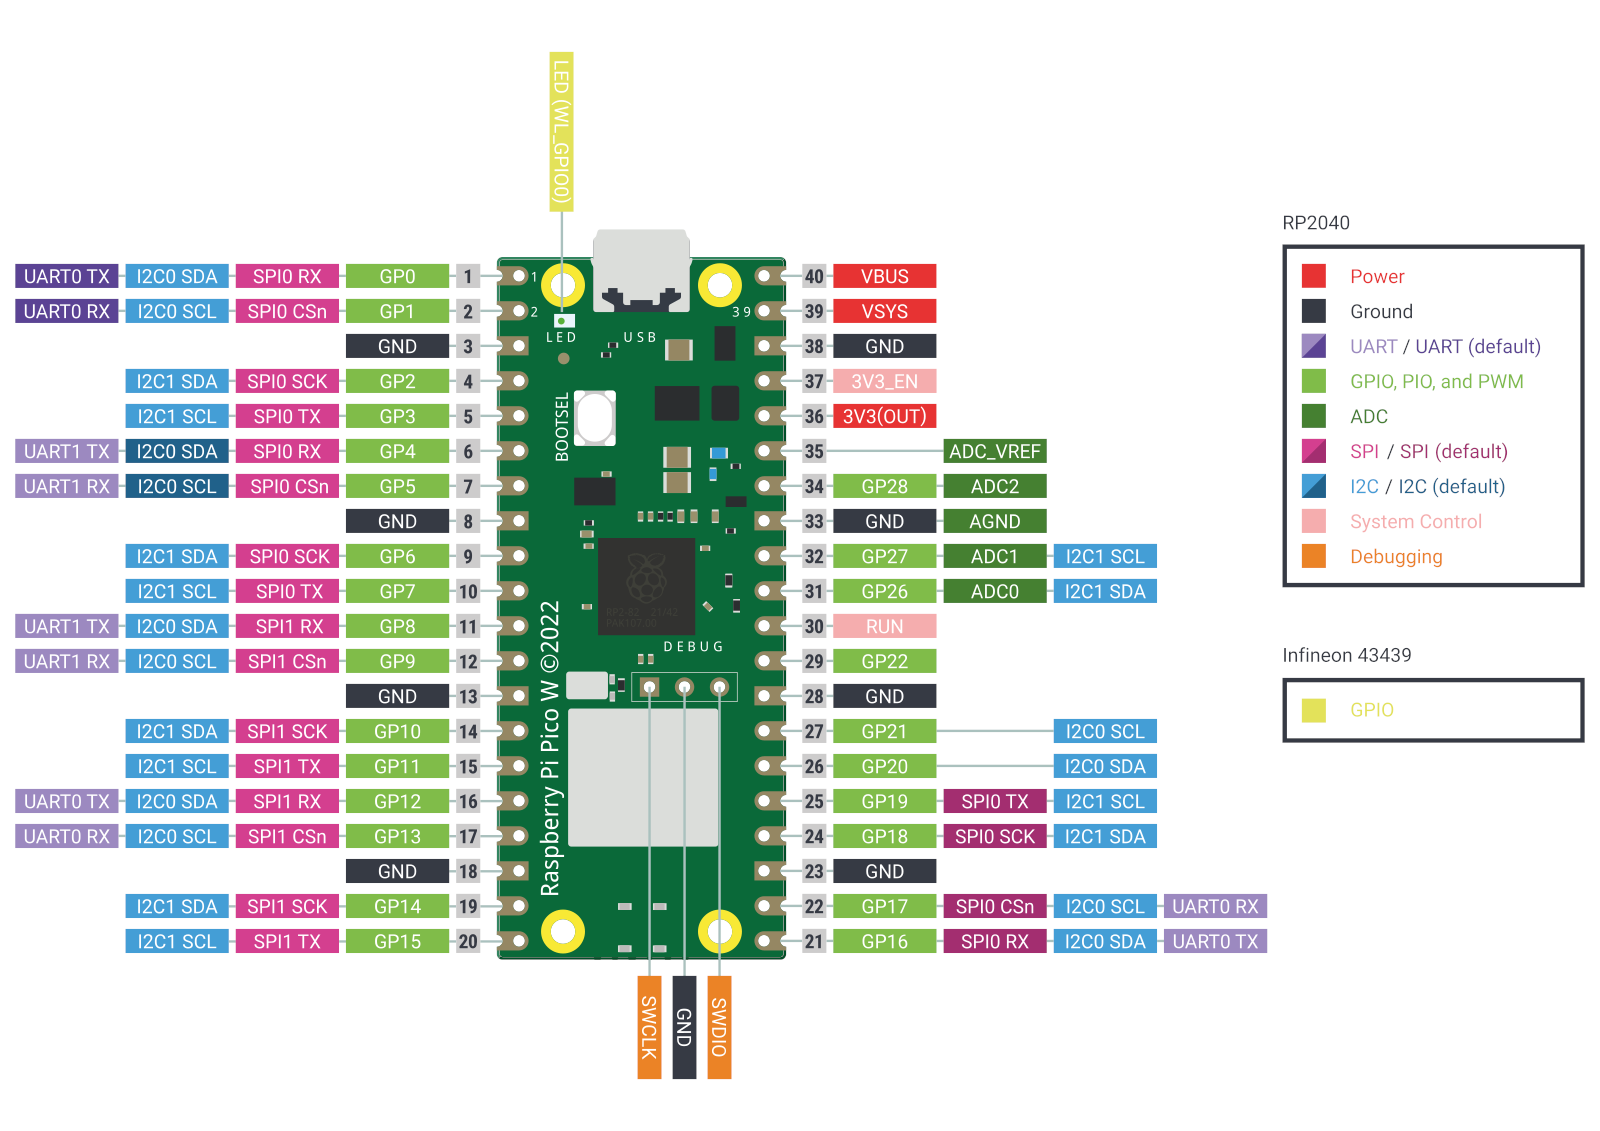
\includegraphics[width=1\textwidth]{img/herramientas/picow.png}
    \caption{Raspberry Pi Pico W Pinout.}
\end{figure}

\begin{figure}[h]
    \centering
    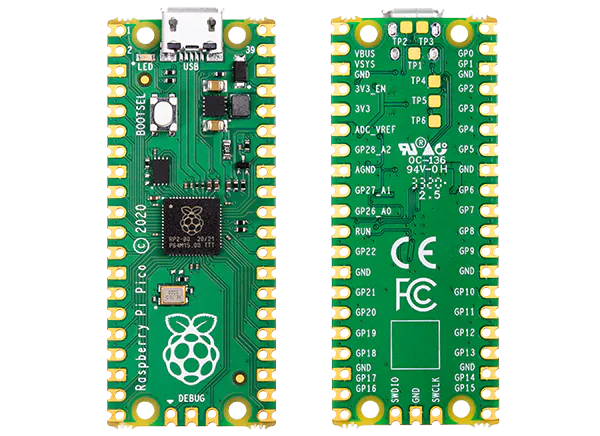
\includegraphics[width=0.5\textwidth]{img/herramientas/picow_vistas.png}
    \caption{Vistas Frontal y posterior de Raspberry Pi Pico W.}
\end{figure}

\pagebreak

\subsection{Pantalla oled I2C de 128x64 píxeles y 1.3 pulgadas}
La pantalla OLED~\cite{manual:Oled} de 128x64 de 1.3 pulgadas con interfaz I2C es un dispositivo de visualización que utiliza la tecnología OLED (Diodo Orgánico de Emisión de Luz) y se comunica a través del protocolo I2C (Inter-Integrated Circuit).

\begin{table}[htbp]
\begin{center}
\caption{Características de la pantalla oled}
\begin{tabular}{|l|l|}
\hline
\rowcolor[HTML]{C0C0C0} 
\textbf{Característica} & \textbf{Descripción}\\ \hline
Voltaje de operación & 3V\quad-\quad5.5 V DC\\ \hline
Interfaz & I2C\\ \hline
Resolución & 128\times64\\ \hline
Monócromo & píxeles blancos (fondo negro)\\ \hline
Ángulo de visión & 160^\circ \\ \hline
Área visicle (display) & 23$\times$11.5 mm\\ \hline
Consumo de energía ultra bajo & 0.08 W (cuando están encendidos todos los píxeles)\\ \hline
item Temperatura de trabajo & -30\textcelsius\quad -\quad70\textcelsius \\ \hline
item Dimensiones & 27\times 27$\times$4.1mm \\ \hline
item Peso & 5 gramos \\ \hline
\end{tabular}
\end{center}
\end{table}

\begin{figure}[h]
    \centering
    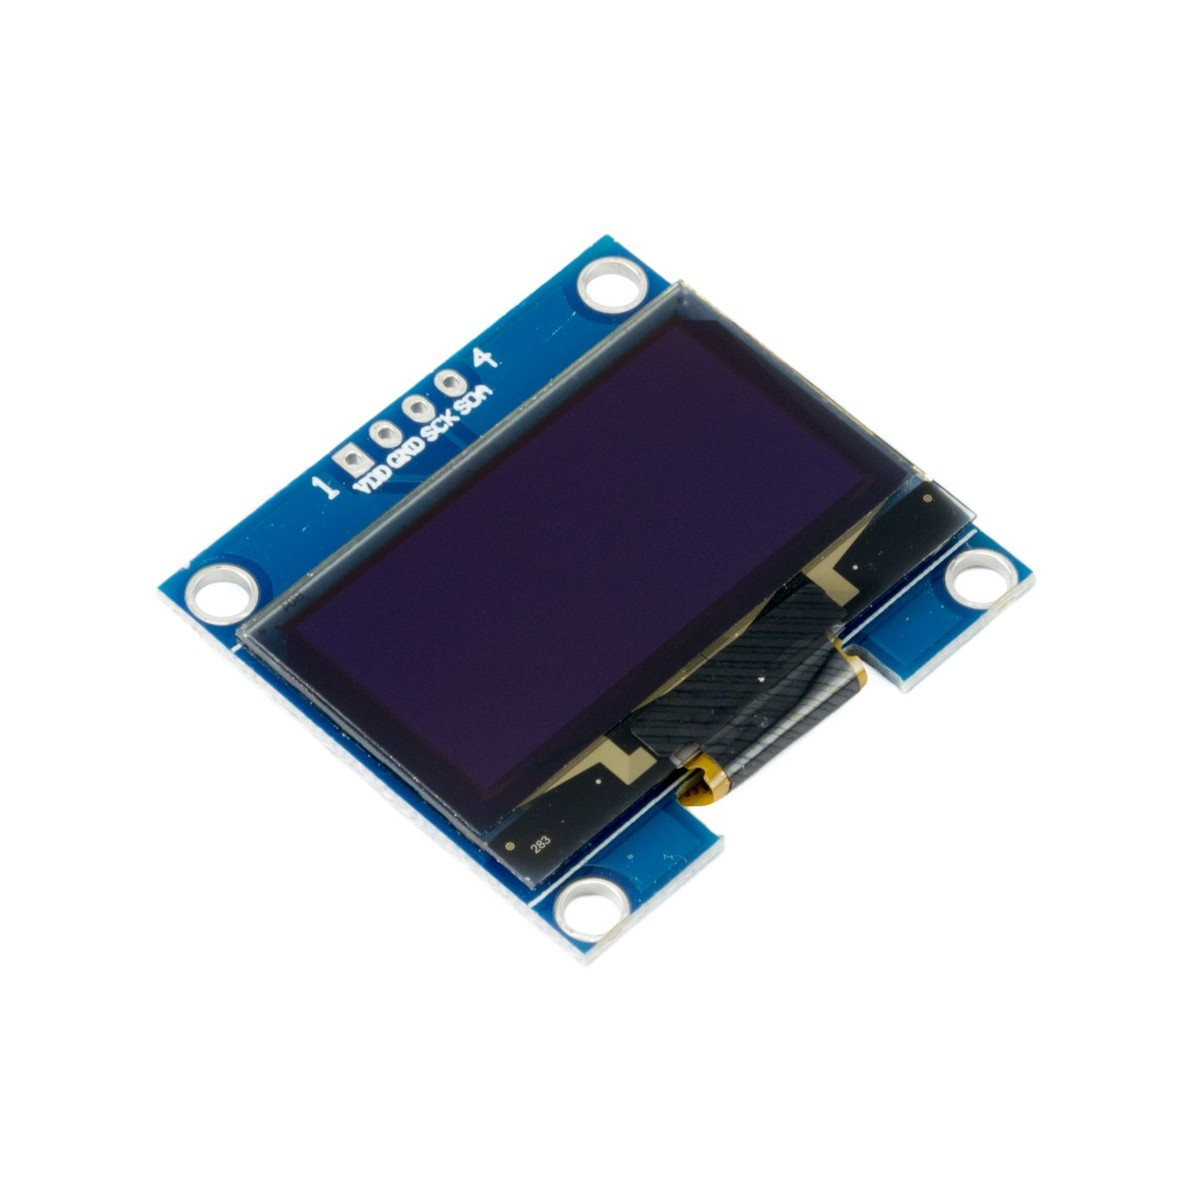
\includegraphics[width=0.5\textwidth]{img/herramientas/oled_cara.png}
    \caption{Pantalla oled.}
\end{figure}

%\begin{figure}[h]
    %\centering
    %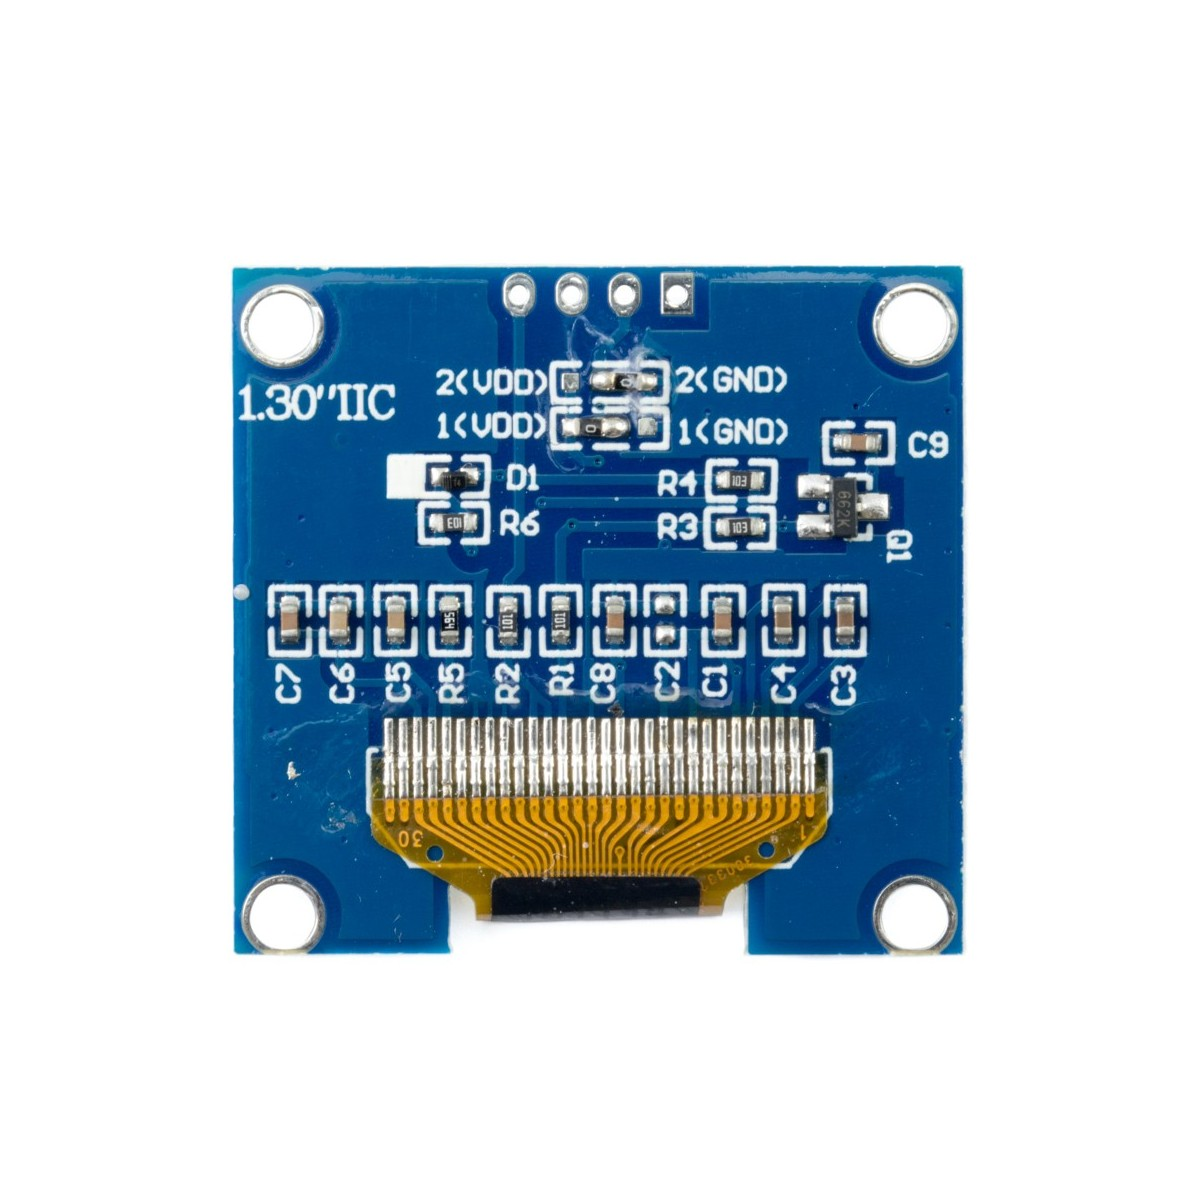
\includegraphics[width=0.5\textwidth]{img/herramientas/oled_reverso.png}
    %\caption{Vista posterior de la pantalla oled.}
%\end{figure}
\pagebreak

\subsection{Sensor de luz BH1750}

El sensor BH1750~\cite{manual:BH1750} es un sensor de intensidad de luz digital que mide la luminosidad ambiental en lux (lx). Este dispositivo es utilizado comúnmente en aplicaciones donde se requiere monitoreo de la luz, como en sistemas de iluminación automática, dispositivos de ahorro de energía y proyectos de IoT.
Posee un conversor interno de 16-bit, por lo que entrega una salida digital en formato I2C

\begin{table}[htbp]
\begin{center}
\caption{Características del sensor de luz BH1750.}
\begin{tabular}{|l|l|}
\hline
\rowcolor[HTML]{C0C0C0} 
\textbf{Característica} & \textbf{Descripción}\\ \hline
Voltaje de Operación &  3V – 5V \\ \hline
Interfaz digital & I2C \\ \hline
Respuesta espectral & similar a la del ojo humano \\ \hline
Rango de medición & 1 lux\quad-\quad65535 lux \\ \hline
Consumo de energía & bajo \\ \hline
\end{tabular}
\end{center}
\end{table}

\begin{figure}[h]
    \centering
    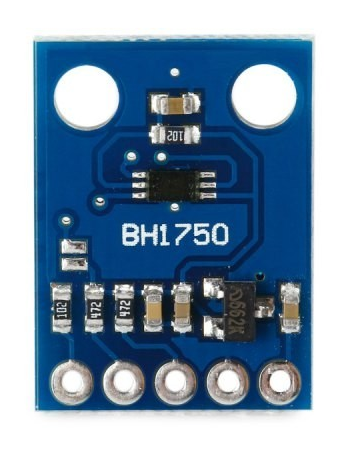
\includegraphics[width=0.4\textwidth]{img/herramientas/bh1750_cara.png}
    \caption{Vista frontal del sensor BH1750.}
\end{figure}
\pagebreak

\begin{figure}[h]
    \centering
    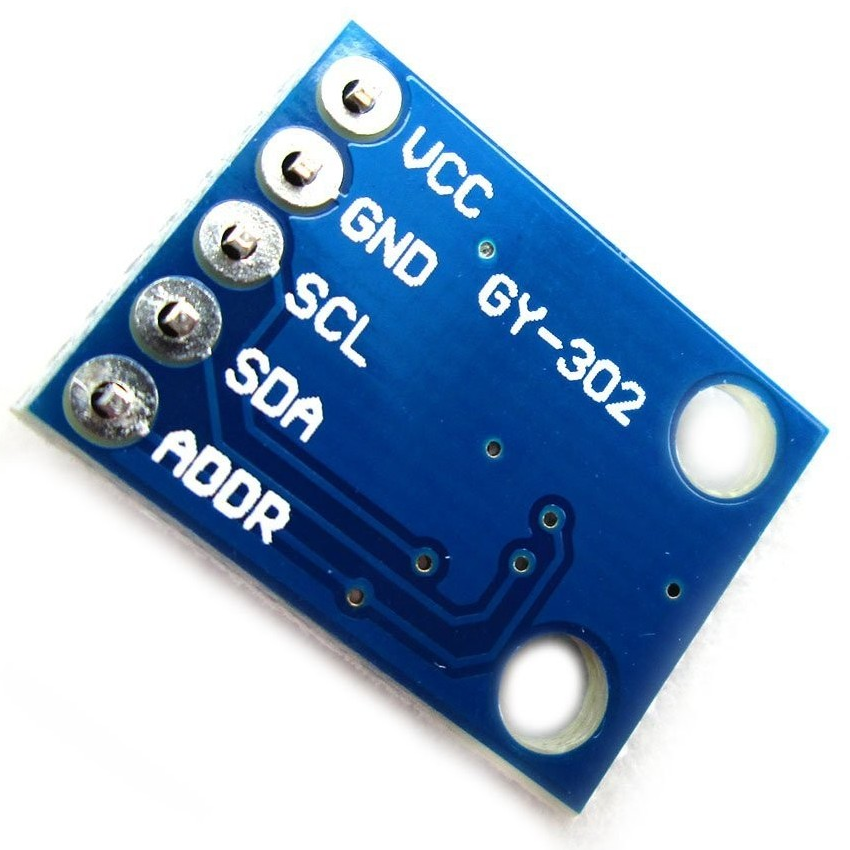
\includegraphics[width=0.4\textwidth]{img/herramientas/bh1750_reverso.png}
    \caption{Lado posterior del sensor BH1750.}
\end{figure}
\pagebreak

\subsection{Sensor de temperatura y humedad DHT22}
El sensor DHT22~\cite{manual:DHT22} (también conocido como AM2302) es un sensor de temperatura y humedad digital utilizado en aplicaciones donde es crucial monitorear y medir las condiciones ambientales.

\begin{table}[htbp]
\begin{center}
\caption{Características del sensor de temperatura y humedad DHT22.}
\begin{tabular}{|l|l|}
\hline
\rowcolor[HTML]{C0C0C0} 
\textbf{Característica} & \textbf{Descripción}\\ \hline
Voltaje de funcionamiento &  3 V\quad-\quad 5.5 V \\ \hline
Forma de salida de señal & señal digital \\ \hline
Rango de medición de temperatura & -40 \textcelsius\quad -\quad 80 \textcelsius  \\ \hline
Rango de medición de humedad & 0\quad-\quad100\% HR \\ \hline
Resolución de temperatura & 0.1 \textcelsius \\ \hline
Resolución de humedad & 0.1\% HR \\ \hline
Precisión de medición de temperatura & $\pm$0.5 \textcelsius \\ \hline
Precisión de medición de humedad & \pm 2$\%$ $ HR$ \\ \hline
Tamaño & 28.2 x 13.1 x 10 mm \\ \hline
Tiempo de sensado & 2s \\ \hline
Modelo & AM2302 \\ \hline
\end{tabular}
\end{center}
\end{table}
\begin{figure}[h]
    \centering
    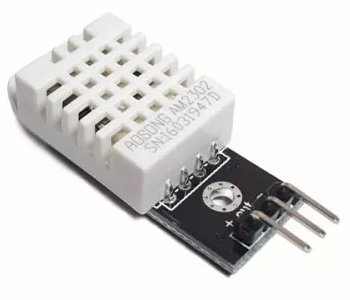
\includegraphics[width=0.7\textwidth]{img/herramientas/dht22.png}
    \caption{Sensor DHT22.}
\end{figure}

\subsection{Sensor de humedad de suelo}
El sensor de humedad de suelo Higrometro V1.2~\cite{wiki:SensorHumedadSuelo} es un dispositivo diseñado para medir la humedad del suelo en entornos agrícolas, de jardinería u otros contextos donde el control de la humedad del suelo es esencial.

\begin{table}[htbp]
\begin{center}
\caption{Características del sensor de humedad de suelo.}
\begin{tabular}{|l|l|}
\hline
\rowcolor[HTML]{C0C0C0} 
\textbf{Característica} & \textbf{Descripción}\\ \hline
Voltaje de alimentación & 3.3V\quad-\quad5V DC \\ \hline
Corriente operación & 5 mA \\ \hline
Voltaje de la señal de salida & 0 a 5V (Analógico) \\ \hline
Modelo & capacitive soil moisture sensor v1.2 \\ \hline
Vida útil & 3 años mínimo \\ \hline
Conector & PH2.0-3P \\ \hline
Dimensiones & 98$\times$23 mm \\ \hline
Peso & 15 gramos \\ \hline
\end{tabular}
\end{center}
\end{table}

\begin{figure}[h]
    \centering
    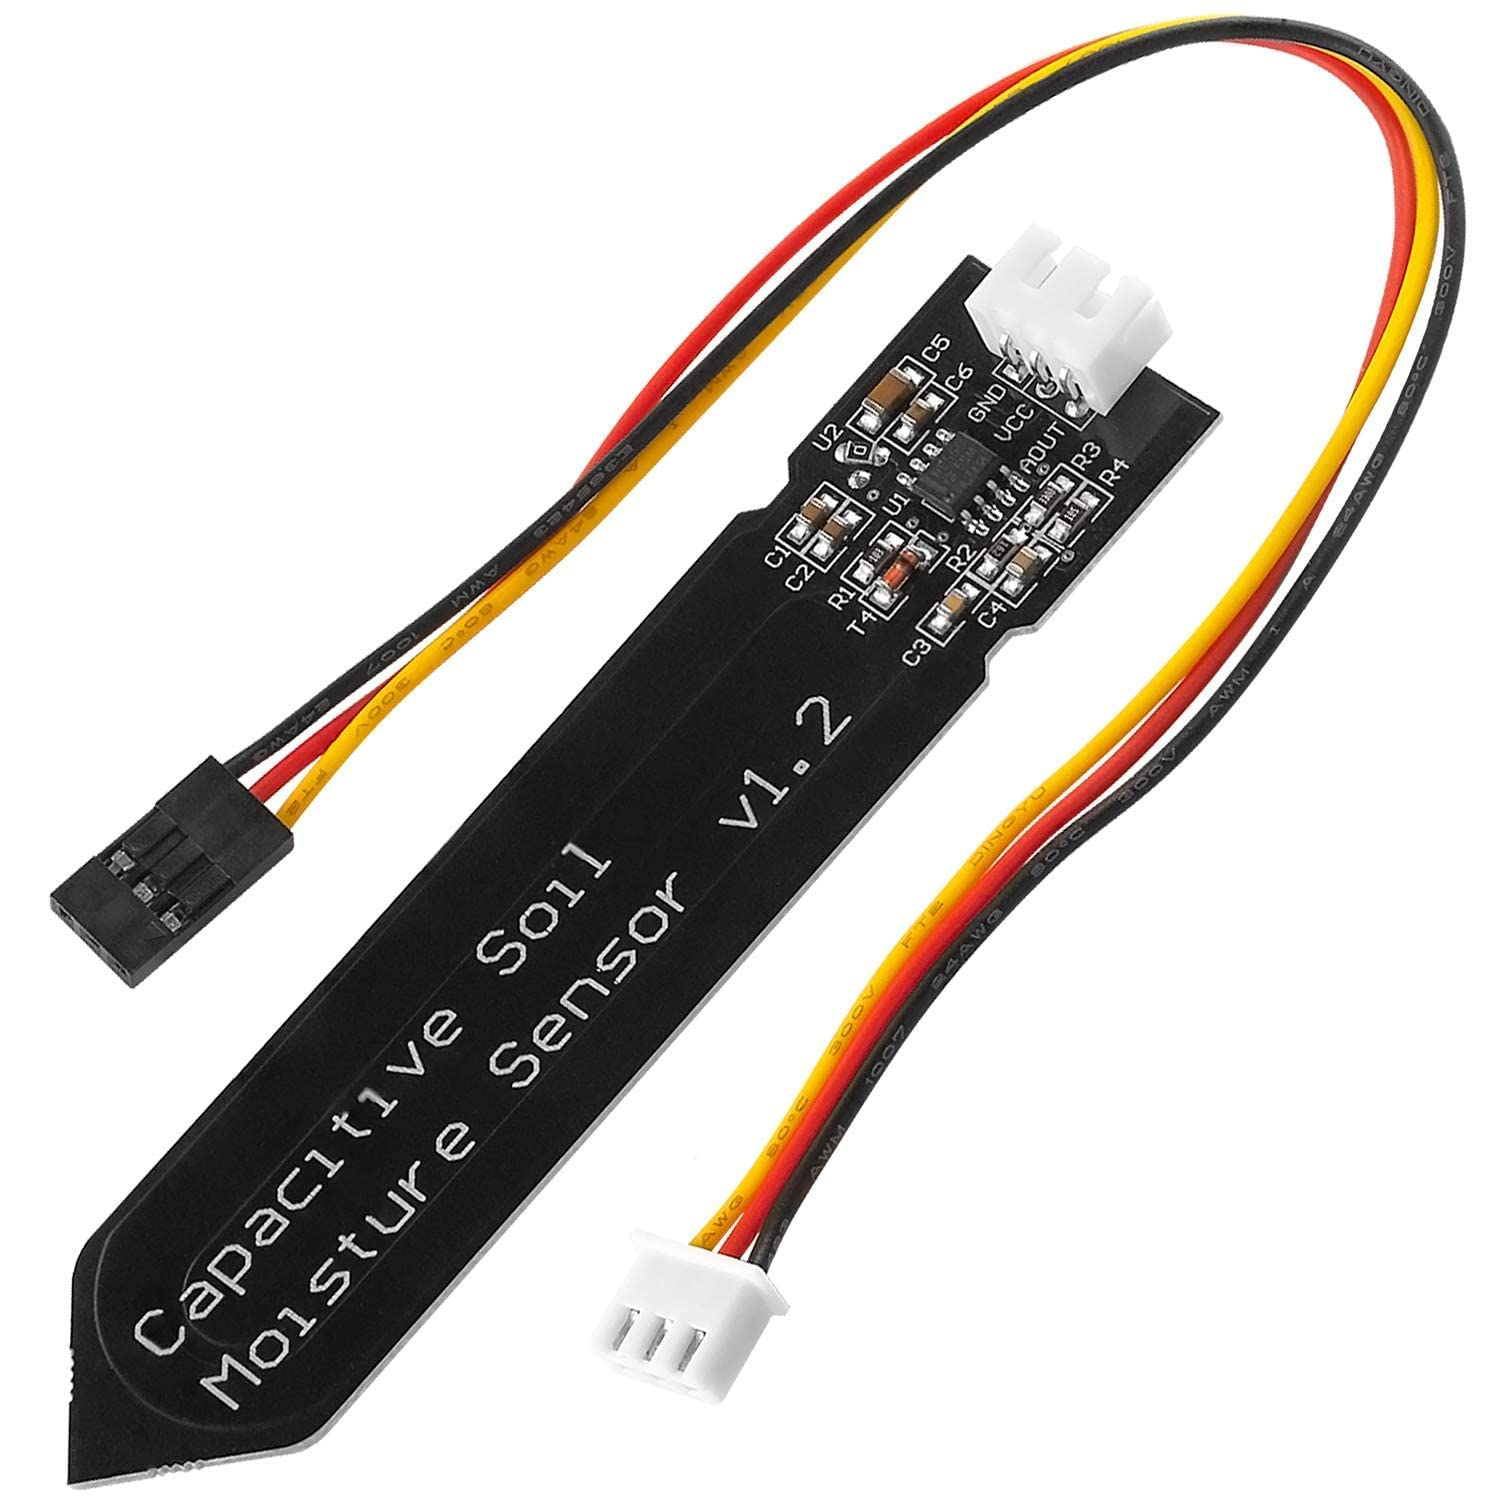
\includegraphics[width=0.7\textwidth]{img/herramientas/SensorHumedadSuelo.png}
    \caption{Sensor de humedad de suelo Higrometro V1.2.}
\end{figure}

\subsection{KY-016 FZ0455 Módulo led RGB de 3 colores}
El módulo KY-016~\cite{manual:LedRGB} FZ0455 es un dispositivo electrónico que contiene un LED RGB (Light Emitting Diode - Diodo Emisor de Luz) capaz de emitir luz en tres colores primarios: rojo, verde y azul. Este módulo se utiliza comúnmente en proyectos electrónicos y de iluminación para agregar efectos de luz y color controlables

\begin{table}[htbp]
\begin{center}
\caption{Características del módulo led RGB KY-016.}
\begin{tabular}{|l|l|} %|c|c|
\hline
\rowcolor[HTML]{C0C0C0} 
\textbf{Característica} & \textbf{Descripción}\\ \hline
Voltaje operativo & 3.3 V\quad5 V\\ \hline
Modo de accionamiento led & Accionamiento de cátodo común \\ \hline
Tamaño & 3.5$\times$0.8 cm\\ \hline
Voltaje de avance V_{f}[Red] & 1.8 V \\ \hline
Voltaje de avance V_{f}[Green, Blue] & 2.8 V \\ \hline
Corriente directa hacia adelante I_{f} & 20 mA \\ \hline
\end{tabular}
\end{center}
\end{table}

\begin{figure}[h]
    \centering
    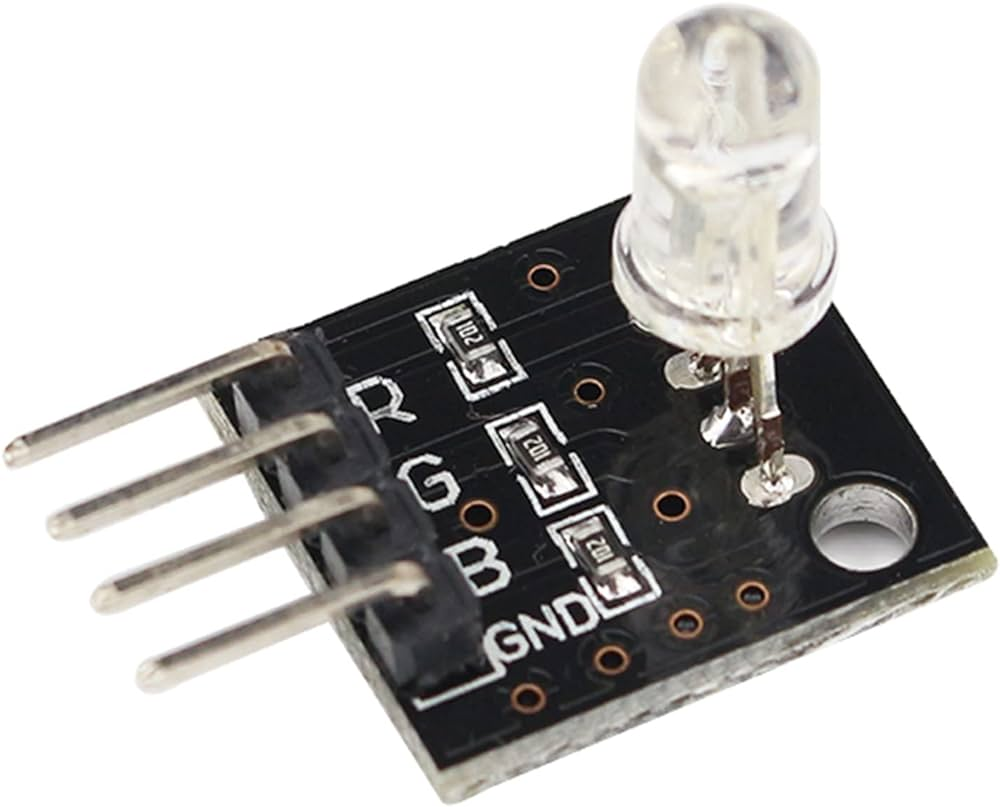
\includegraphics[width=0.8\textwidth]{img/herramientas/LedRGB.png}
    \caption{Módulo led RGB KY-016.} \label{Img:LedRGB}
\end{figure}

\subsection{Enrutador WiFi USB 4G LTE}
El Enrutador WiFi~\cite{misc:EnrutadorWifi} USB 4G LTE es un dispositivo portátil que permite establecer una conexión a Internet de alta velocidad utilizando la red móvil 4G LTE. Diseñado para la movilidad y la conveniencia, este router WiFi ofrece una solución eficiente para aquellos que requieren acceso a la red en cualquier lugar donde haya cobertura de red móvil. Con una ranura para tarjeta SIM, el dispositivo facilita la inserción de una tarjeta SIM compatible, lo que lo convierte en una opción versátil para la conectividad a Internet en movimiento. Con una velocidad de transferencia de hasta 150 Mbps, este enrutador proporciona un rendimiento adecuado para actividades en línea como navegación web, transmisión de video y juegos en línea.

\begin{table}[htbp]
\begin{center}
\caption{Características del enrutador WiFi USB 4G LTE.}
\begin{tabular}{|l|l|}
\hline
\rowcolor[HTML]{C0C0C0} 
\textbf{Característica} & \textbf{Descripción}\\ \hline
Velocidad de Transferencia &  Hasta 150 Mbps\\ \hline
Red Móvil Compatible &  Tecnología 4G LTE \\ \hline
4G LTE FDD & B1/B3/B5 \\ \hline
Wifi & Support IEEE802.11b/g/n Band 2.4G \\ \hline
Número máximo de usuarios & 10 \\ \hline
Ranura para Tarjeta SIM &  Necesario para la conexión a la red móvil \\ \hline
Conectividad WiFi & Proporciona una red WiFi local\\ \hline
Compatibilidad & Computadoras, tabletas y teléfonos \\ \hline
Seguridad & Cifrado WPA/WPA2 \\ \hline
Alimentación por batería & Es opcional y permite mayor portabilidad \\ \hline
Indicadores LED & Estado de la conexión e intensidad de la señal \\ \hline
Material & ABS \\ \hline
Dimensiones & 4.33$\times$2.76$\times$0.79 pulgadas\\ \hline
\end{tabular}
\end{center}
\end{table}

\begin{figure}[h]
    \centering
    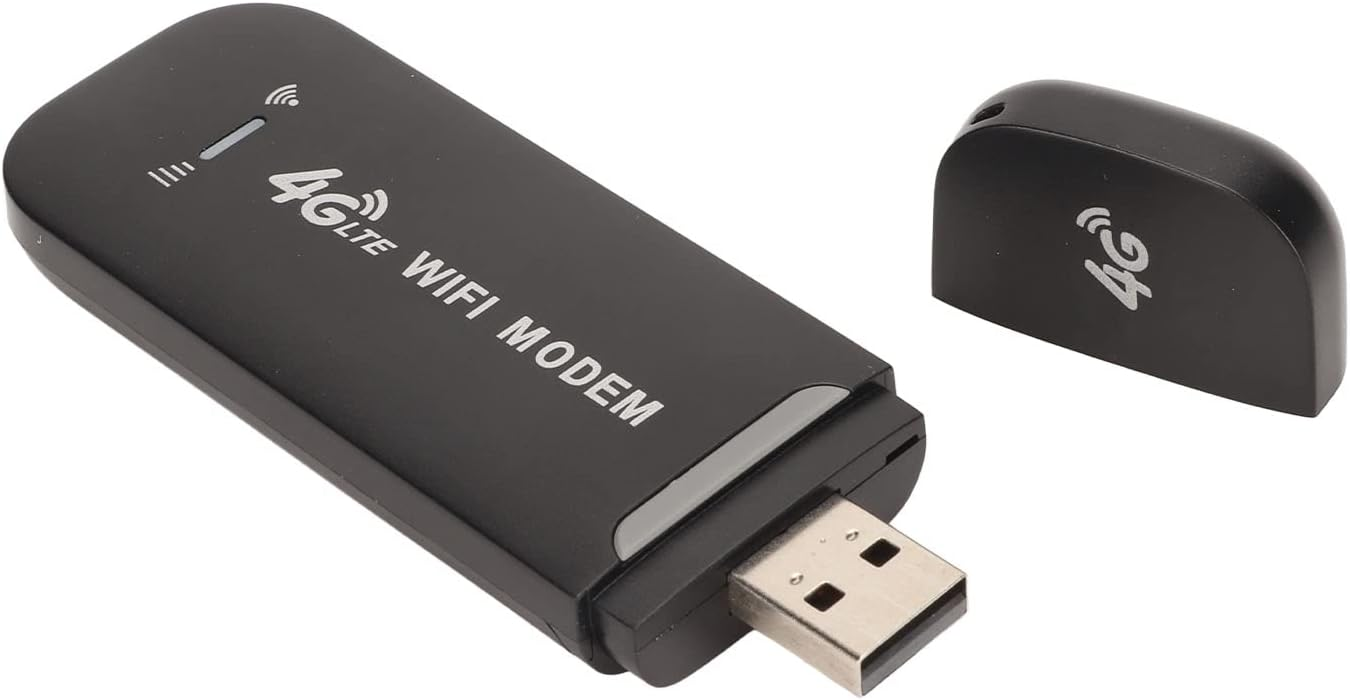
\includegraphics[width=0.5\textwidth]{img/herramientas/enrutador_wifi.png}
    \caption{Enrutador WiFi USB 4G LTE.} \label{Img:EnrutadorWifi}
\end{figure}

\subsection{Batería externa 20000 mAh}
Es un Power Bank~\cite{misc:Powerbank} portátil diseñado para cargar dispositivos móviles de forma rápida y eficiente. Con dos salidas USB-A y una entrada Type-C, proporciona flexibilidad para cargar múltiples dispositivos simultáneamente y recargarse fácilmente. Fabricada con aleación de aluminio, esta mini Powerbank, en elegante color gris, ofrece durabilidad y un diseño compacto que facilita su transporte. Con una capacidad de 20000mAh, es ideal para mantener tus dispositivos cargados mientras estás en movimiento, ya sea en viajes, actividades al aire libre o situaciones de emergencia.

\begin{table}[htbp]
\begin{center}
\caption{Características de la batería externa 20000 mAh.}
\begin{tabular}{|l|l|}
\hline
\rowcolor[HTML]{C0C0C0} 
\textbf{Característica} & \textbf{Descripción}\\ \hline
Tipo de conector entrada & usb tipo C (5V/2A)\\ \hline
Tipo de conector salida & usb tipo A2 (5V/2A)\\ \hline
Marca & YWTESCH \\ \hline
Color & Gris \\ \hline
Tensión & 5 voltios \\ \hline
Amperaje & 2 A \\ \hline
Capacidad máxima & 20000 mAh \\ \hline
Número de puertos & 2 \\ \hline
tamaño & 108$\times$69$\times$26 mm \\ \hline
\end{tabular}
\end{center}
\end{table}

\begin{figure}[h]
    \centering
    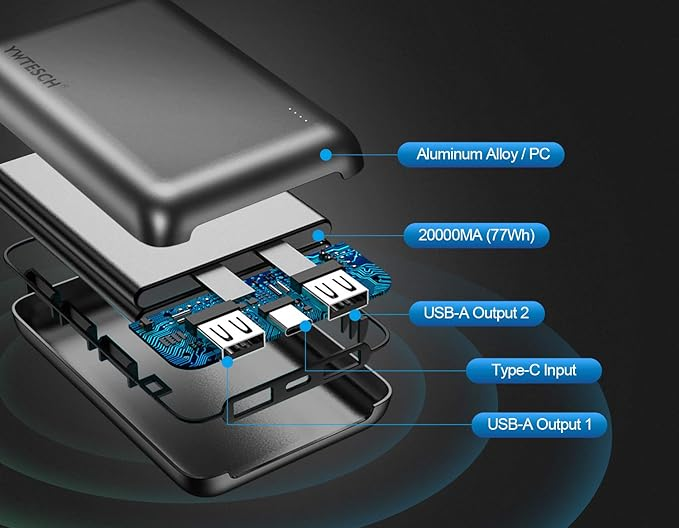
\includegraphics[width=0.6\textwidth]{img/herramientas/bateria_externa_descripcion.png}
    \caption{Batería externa 20000 mAh.} \label{Img:BateriaExterna}
\end{figure}

\subsection{Panel solar IP65 de 8W y 5V con cargador USB tipo C}
Este Panel Solar~\cite{misc:PanelSolar} es una solución eficiente para la carga de dispositivos móviles utilizando energía solar. Es una opción versátil para cargar dispositivos compatibles, como teléfonos, tabletas y otros dispositivos alimentados por USB. Compacto y fácil de transportar, es ideal para actividades al aire libre, viajes y situaciones donde la carga convencional no está disponible.

\begin{table}[htbp]
\begin{center}
\caption{Características del panel solar.}
\begin{tabular}{|l|l|} %|c|c|
\hline
\rowcolor[HTML]{C0C0C0} 
\textbf{Característica} & \textbf{Descripción}\\ \hline
USB & Tipo C con cable de 3 m \\ \hline
Capacidad & 8W y 5V \\ \hline
Material del panel & Silicio monocristalino \\ \hline
Vida útil & 20 años \\ \hline
Accesorios & Soporte ajustable 360$^\circ$ con tornillos y tojinos \\ \hline
Dimensiones & 23$\times$18.5$\times$1 cm\\ \hline
Tipo de protección & IP65 (resistente al polvo y agua)\\ \hline
\end{tabular}
\end{center}
\end{table}

\begin{figure}[h]
    \centering
    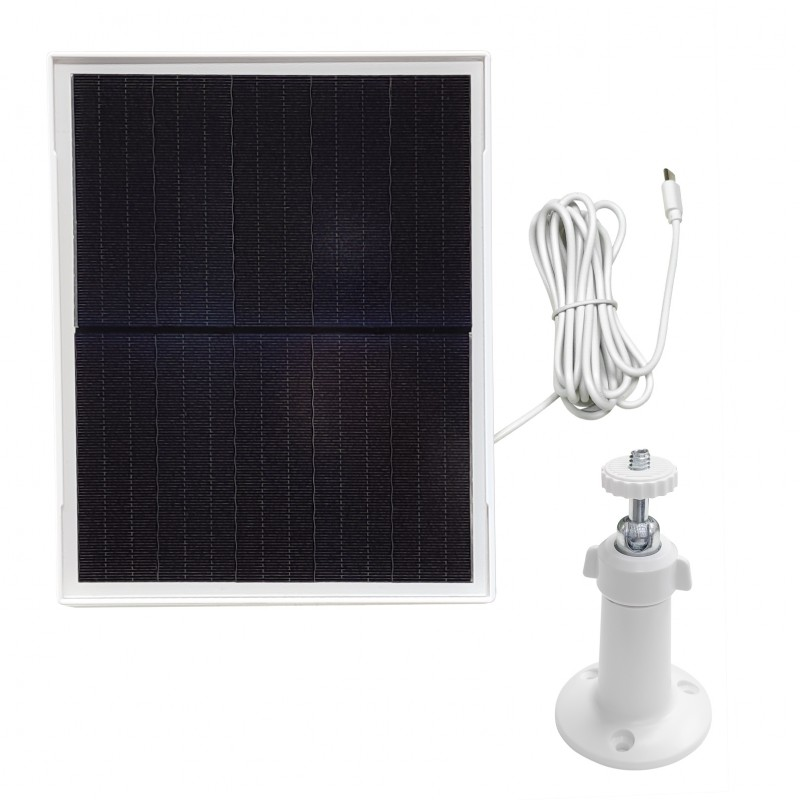
\includegraphics[width=0.7\textwidth]{img/herramientas/panel_solar.png}
    \caption{Panel solar y soporte ajustable.} \label{Img:PanelSolar}
\end{figure}

%Esta parte de la memoria tiene como objetivo presentar las técnicas metodológicas y las herramientas de desarrollo que se han utilizado para llevar a cabo el proyecto. Si se han estudiado diferentes alternativas de metodologías, herramientas, bibliotecas se puede hacer un resumen de los aspectos más destacados de cada alternativa, incluyendo comparativas entre las distintas opciones y una justificación de las elecciones realizadas. 
%No se pretende que este apartado se convierta en un capítulo de un libro dedicado a cada una de las alternativas, sino comentar los aspectos más destacados de cada opción, con un repaso somero a los fundamentos esenciales y referencias bibliográficas para que el lector pueda ampliar su conocimiento sobre el tema.
